\documentclass[a4paper, twoside, english]{article}

\usepackage{amsmath}
\usepackage{amsfonts}
\usepackage{ihci}
\usepackage{graphicx}
\usepackage{subfig}

\graphicspath{{./../figures/}}

\title{Template Report \\ 3D Computer Vision}  % Replace "Template Report" with Exercise 1, Exercise 2, etc
\author{Christiano Gava}                       % Replace with your names
\date{27.11.2017}                              % Replace with current date

\begin{document}

\maketitle

\section{Introduction}

This template is meant to provide basic knowledge in \LaTeX\ for students to achieve the required quality of exercise reports of the lecture 3D Compute Vision.
It is also an opportunity for those not yet familiar with \LaTeX\ to learn this awesome tool.

\section{Basics}

In technical reports as well as in scientific manuscripts it is common to work with equations, figures and citations.
Concerning equations, there are several commands available to format them and produce the desired results.
This template focuses on the basics necessary for the exercise reports.
For instance, Eq.~\ref{eq:projection} shows the standard projection of a 3D point $X \in \mathbb{R}^3$ onto a perspective image as
\begin{equation}
 \begin{aligned}
  \lambda x &= P X \\
          x &\sim K \left[ R | t \right] X,
 \end{aligned}
 \label{eq:projection}
\end{equation}
where $P_{3 \times 4}$ is the projection matrix.
Note the alignement on $=$ and $\sim$; this is very useful to neatly display equations.
Still referring to Eq.~\ref{eq:projection}, $K$ is usually called camera matrix and is given by
\begin{equation*}
 K = \left[
 \begin{array}{ccc}
  f_x & s & c_x \\
  0 & f_y & c_y \\
  0 & 0 & 1
 \end{array}
 \right].
 \label{eq:kmatrix}
\end{equation*}

The matrix $K$ holds the \emph{intrinsic} camera parameters whereas the rotation matrix $R_{3 \times 3}$ and the translation vector $t_{3 \times 1}$ hold the \emph{extrinsic} parameters, that is, 
they describe the camera pose as shown in Figure~\ref{fig:stdProj}.
\begin{figure}[ht]
 \centerline{
\includegraphics[width=0.65\textwidth]{stdProjection.png}}
 \caption[Standard perspective projection]{Standard perspective projection.}
 \label{fig:stdProj}
\end{figure}

\LaTeX\ also offers convenient ways to arrange multiple pictures into a single figure.
Figure~\ref{fig:inversion} shows an example where an image and the result of processing it are displayed side by side.
\begin{figure}[ht]
 \centerline
 {
  \subfloat[]{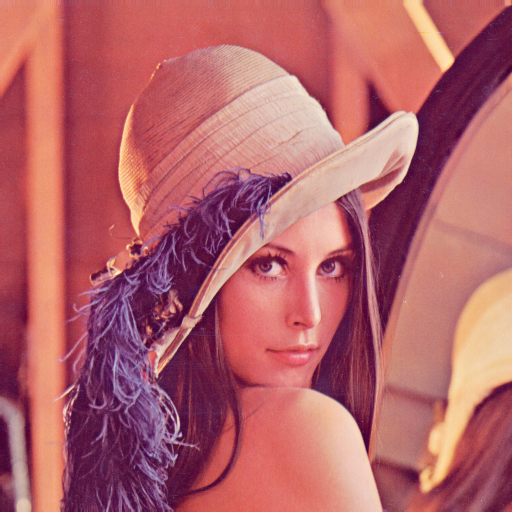
\includegraphics[width=0.35\textwidth]{lena.png}}
  \qquad
  \subfloat[]{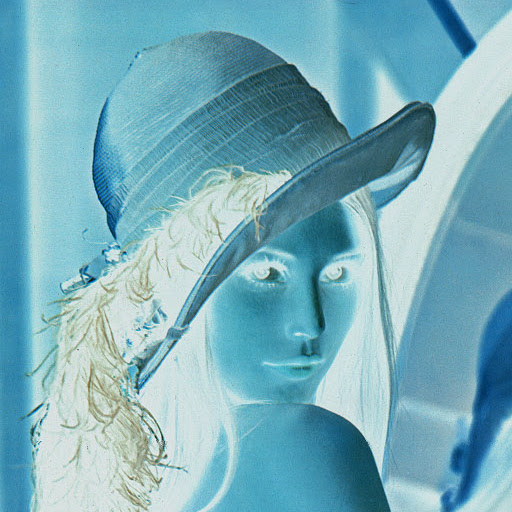
\includegraphics[width=0.35\textwidth]{lenaInverted.png}}
 }
 \caption[Color inversion]{(a) Original image. (b) Result of inverting the colors of (a).}
 \label{fig:inversion}
\end{figure}

Citations are also straightforward.
For example, one of the text books adopted in this lecture can be found in~\cite{Hartley2004}.

\section{Software}

\subsection{PDF Viewer}
In principle, any pdf viewer will do.
For those who prefer to work with DVI files before creating the final pdf version, Okular (\url{https://okular.kde.org/}) may be a good choice.
DVI files~\footnote{DVI files are specially interesting when working with large documents since the generation of the pdf version may take some time.} are generated quickly and may be seen as an 
intermediate stage between the source file (.tex) and the pdf.

\subsection{Editors}
There are many flavors.
Here are some:
\begin{itemize}
 \item Texmaker (Linux, Windows, Mac);
 \item TeXstudio (Linux, Windows, Mac);
 \item MiKTeX (Windows);
 \item \textbf{Kile} (KDE Linux)
\end{itemize}

\subsection{Image format}
It is recommended to work with either \texttt{png} or \texttt{eps} format.
If you choose the former, beware the generation of DVI files will most likely fail.
In this case, you will need to invoke PDFLatex, which converts the source file directly to pdf.
If you prefer \texttt{eps}, creating DVI files should work smoothly.

\bibliographystyle{plain}
\bibliography{bibliography.bib}
\end{document}